\documentclass[tikz,border=2mm]{standalone}
\begin{document}
	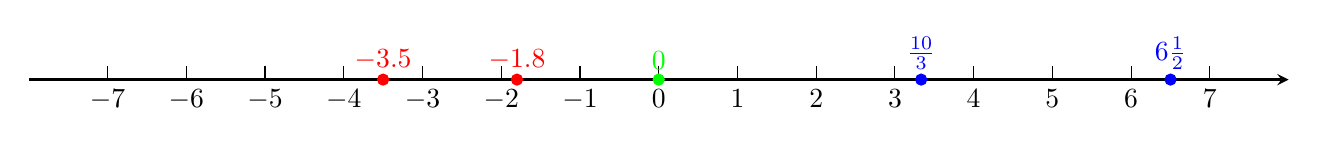
\begin{tikzpicture}
  		\draw [black, thick, ->, >=stealth] (-8,0) -- (8,0); % ->��ͷ��,>=stealth��ʵ�ļ�ͷ
		%\foreach \x in {-9, -8, -7, -6, -5, -4, -3, -2, -1, 0, 1, 2, 3, 4, 5, 6, 7, 8, 9}
		\foreach \x in {-7, ..., 7}
			\draw (\x cm,5pt) -- (\x cm,0pt) node[anchor=north] {$\x$};
		% -1.8, 0, -3.5, 10/3, 6+1/2
		\draw [red, fill=red] (-1.8, 0) circle(2pt) node [above] {$-1.8$}; 
		\draw [red, fill=red] (-3.5, 0) circle(2pt) node [above] {$-3.5$}; 
		\draw [green, fill=green] (0, 0) circle(2pt) node [above] {$0$}; 		
		\draw [blue, fill=blue] (10/3, 0) circle(2pt) node [above] {$\frac{10}{3}$}; 
		\draw [blue, fill=blue] (6+1/2, 0) circle(2pt) node [above] {$6\frac{1}{2}$}; 		
	\end{tikzpicture}    
\end{document}
